\chapter{Switch Interfaces}\label{switch-interfaces}

\begin{figure}
\centering
\pandocbounded{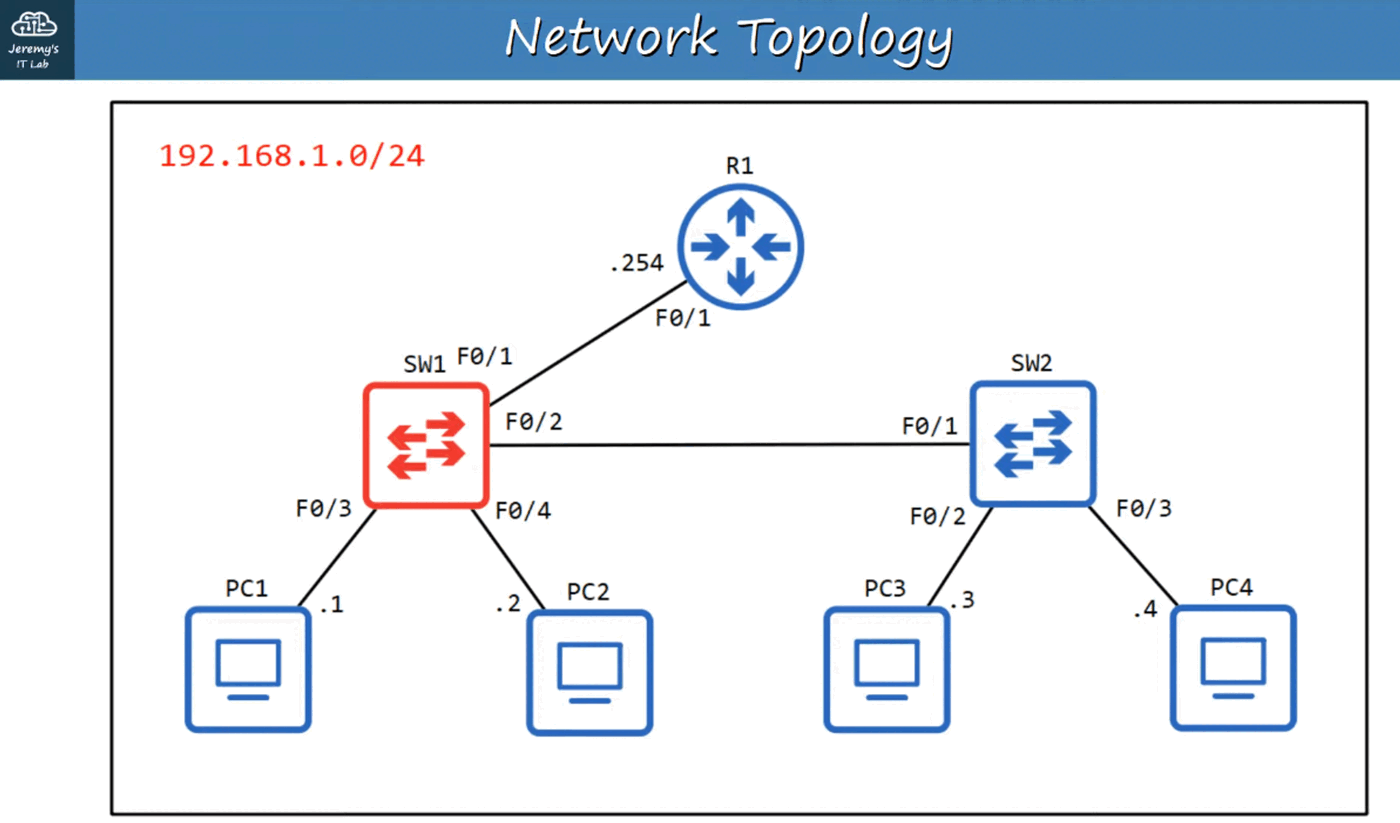
\includegraphics[keepaspectratio,alt={image}]{images/09-switch-interfaces/img-001.png}}
\end{figure}

CISCO CLI for SWITCHES

\begin{figure}
\centering
\pandocbounded{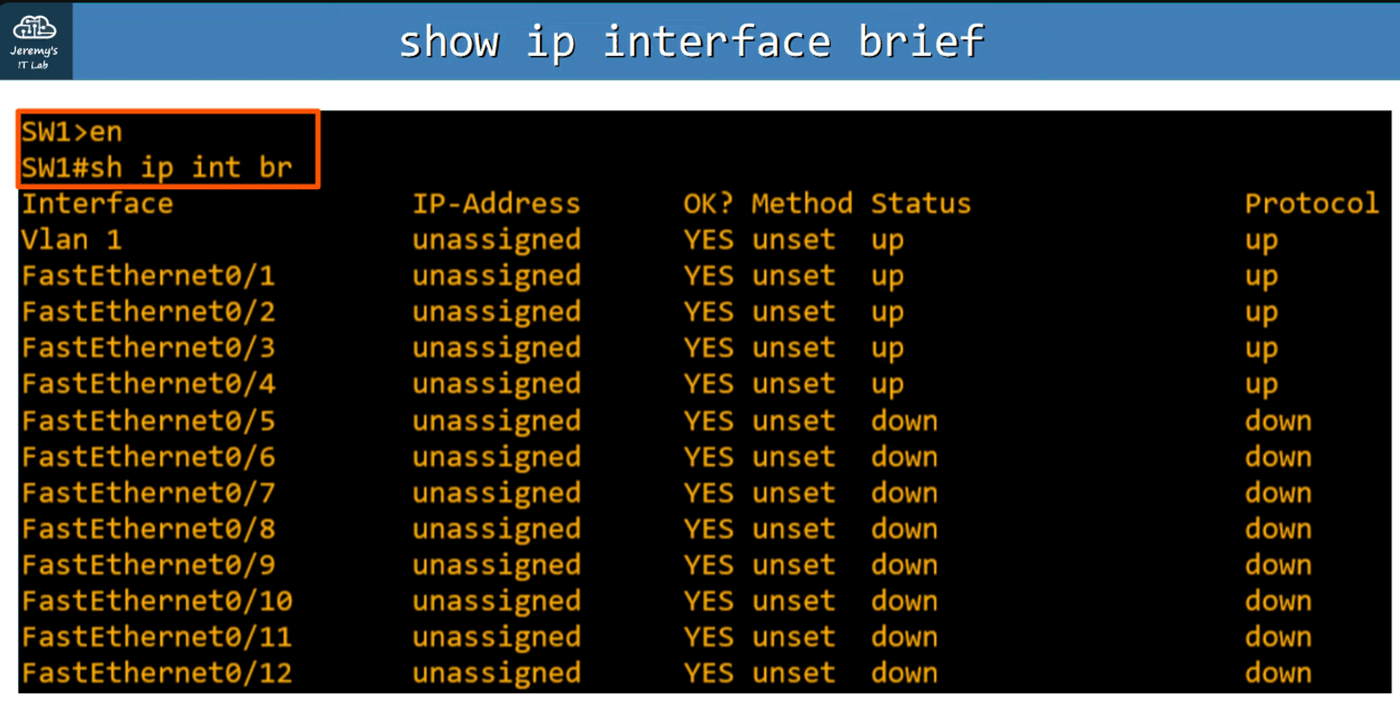
\includegraphics[keepaspectratio,alt={image}]{images/09-switch-interfaces/img-002.png}}
\end{figure}

// enter Privileged EXEC mode

SW1\textgreater enable

// Show all interfaces of Switch 1.

SW\# show ip interface brief

This will show the interfaces currently on Switch 1. It has the same
information structure as Cisco Routers.

Notice the Status (Layer 2) and Protocol (Layer 1) columns are showing
``up/up''.

Unlike ROUTERS, SWITCHES do no DEFAULT to `administrative
down/down'(shutdown).

Unconnected devices will show as ``down'' and ``down'' (not connected to
another device)

\begin{figure}
\centering
\pandocbounded{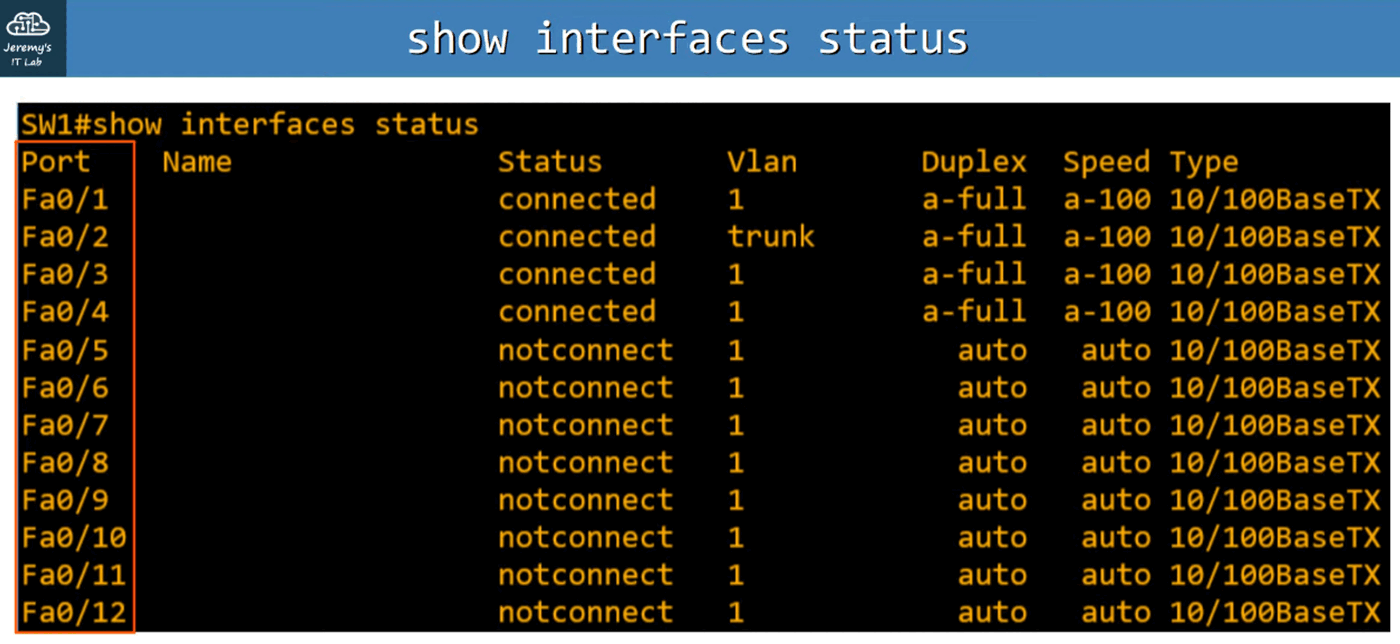
\includegraphics[keepaspectratio,alt={image}]{images/09-switch-interfaces/img-003.png}}
\end{figure}

// Show the status of all interfaces on SW1

SW1\#show interfaces status

This will list:

\begin{itemize}
\tightlist
\item
  Ports
\item
  Name (which is description)
\item
  Status (connection status)
\item
  Vlan (can be used to divide up LANs) - Vlan 1 is the default.
\item
  Duplex (can the connection send/receive at same time?) - Auto is
  default
\item
  Speed (speed in bps) - Auto is default
\item
  Type (what medium is being used, speed of interface)
\end{itemize}

\begin{figure}
\centering
\pandocbounded{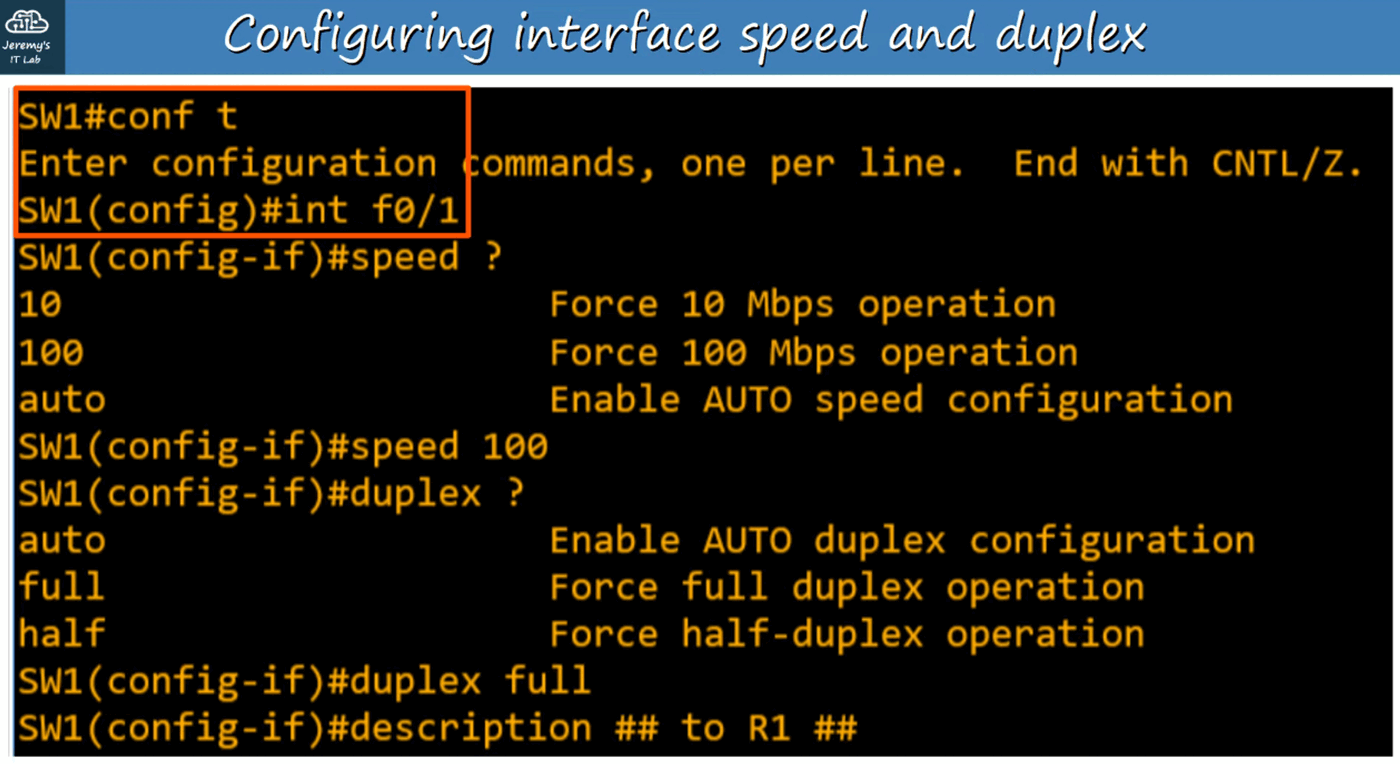
\includegraphics[keepaspectratio,alt={image}]{images/09-switch-interfaces/img-004.png}}
\end{figure}

\begin{figure}
\centering
\pandocbounded{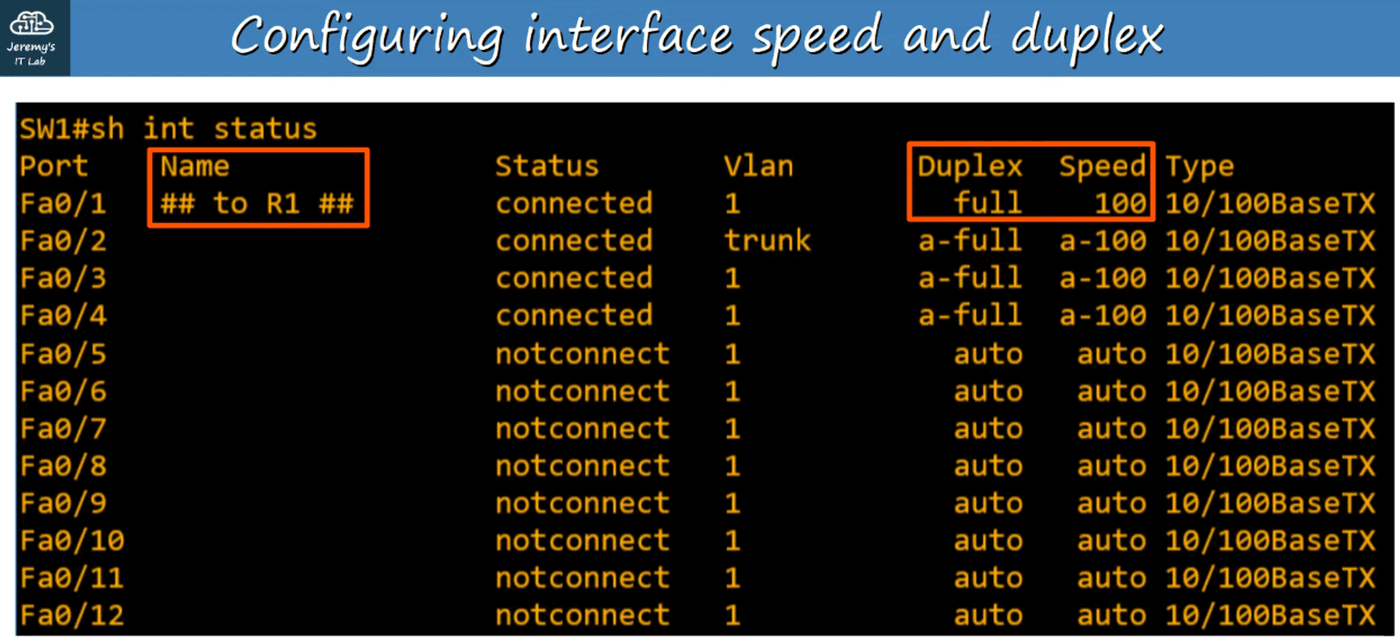
\includegraphics[keepaspectratio,alt={image}]{images/09-switch-interfaces/img-005.png}}
\end{figure}

\section{Interface Range}\label{interface-range}

Unused Interfaces can pose a security risk so it's a good idea to
deactivate them.

However, if you have 28+ interfaces not in use, do you have to do them
one at a time?

Answer: No! There is a command to apply configurations to a range of
interfaces.

Inside Global Config Mode (config t):

\begin{figure}
\centering
\pandocbounded{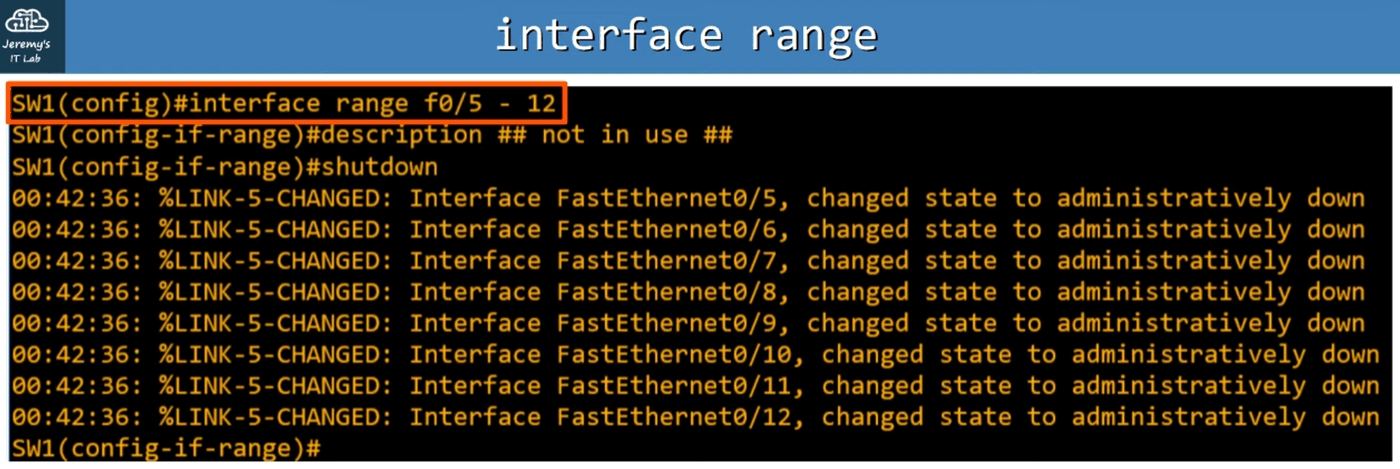
\includegraphics[keepaspectratio,alt={image}]{images/09-switch-interfaces/img-006.png}}
\end{figure}

SW1(config)\#interface range f0/5 - 12 // Choose all interfaces from 0/5
to 0/12

SW1(config-if-range)\#description \#\# not in use \#\#

SW1(config-if-range)\#shutdown

\textless\textless{} this will list all the interfaces being set to
administratively down \textgreater\textgreater{}

Confirm with `show interface status' in Privileged EXEC mode or if in
CONFIG mode, use `do show interface status'

\begin{figure}
\centering
\pandocbounded{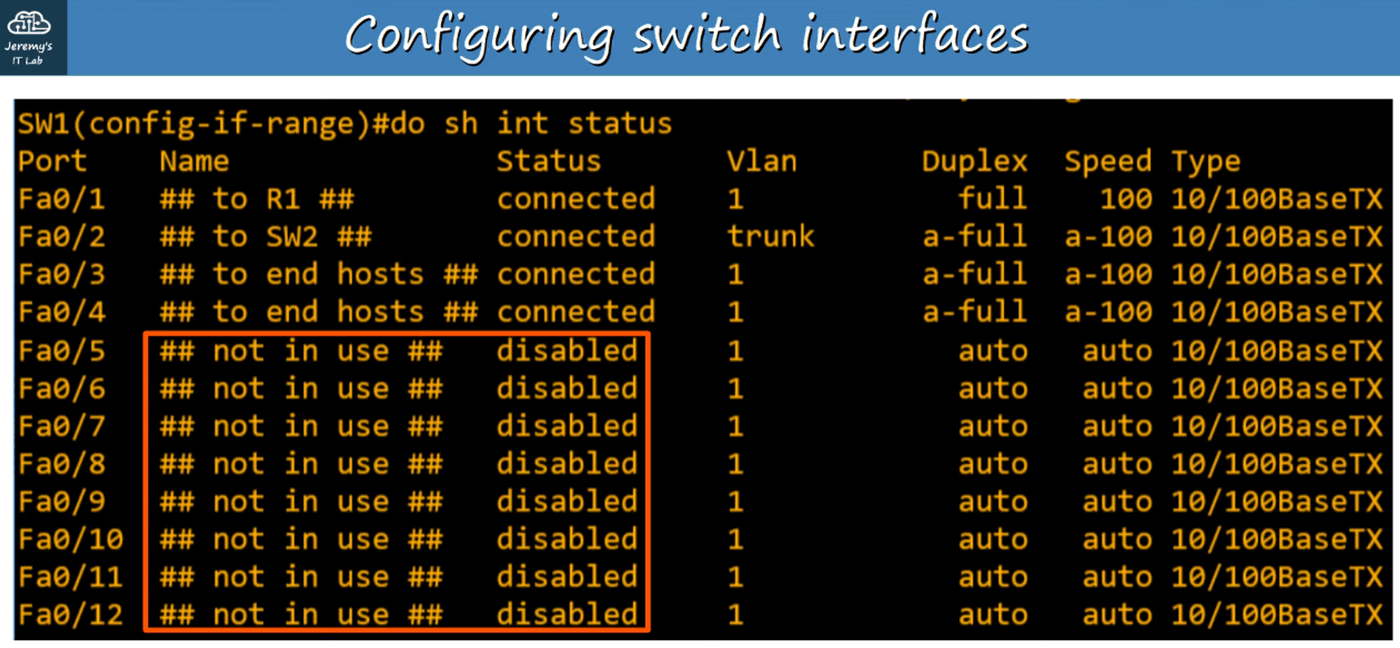
\includegraphics[keepaspectratio,alt={image}]{images/09-switch-interfaces/img-007.png}}
\end{figure}

\section{Full / Half Duplex}\label{full-half-duplex}

\section{Half Duplex}\label{half-duplex}

\begin{itemize}
\tightlist
\item
  Device cannot send / receive data at the same time. If it is receiving
  a frame, it must wait before sending a frame.
\end{itemize}

\section{Full Duplex}\label{full-duplex}

\begin{itemize}
\tightlist
\item
  Device CAN send / receive data at the same time. It does NOT have to
  wait.
\end{itemize}

MOST modern SWITCHES support FULL DUPLEX.

WHERE is HALF DUPLEX used? Almost nowhere.

In the past, LAN HUBS used HALF DUPLEX.

When multiple packets were received by the HUB, the HUB would simple
FLOOD the connections with frame data, causing a COLLISION (on the
interface), and hosts would not receive the frame intact.

All devices connected to a HUB are called a COLLISION DOMAIN.

To DEAL with COLLISIONS, Ethernet devices use a mechanism called
CSMA/CD.

CSMA/CD = CARRIER SENSE MULTIPLE ACCESS with COLLISION DETECTION.

\begin{itemize}
\tightlist
\item
  Before sending frames, devices `listen' to the collision domain until
  they detect that other devices are not sending.
\item
  IF a collision occurs, the device sends a jamming signal to inform the
  other devices that a collision happened.
\item
  Each device will wait a random period of time before sending frames
  again.
\item
  The process repeats.
\end{itemize}

SWITCHES are more sophisticated than HUBS.

HUBS are Layer 1 Devices - Collisions are common and use CSMA/CD.
SWITCHES are Layer 2 Devices - Collisions RARELY occur.

\begin{figure}
\centering
\pandocbounded{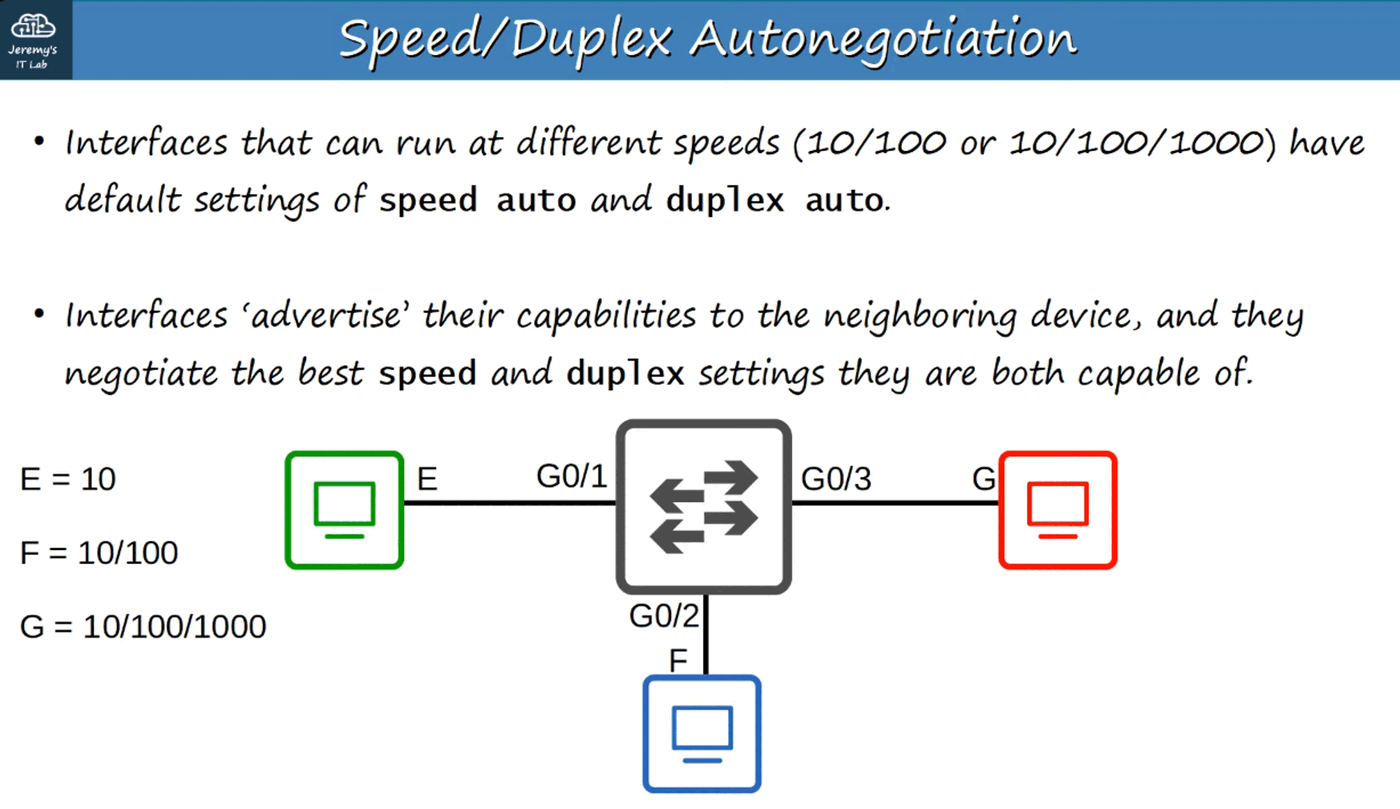
\includegraphics[keepaspectratio,alt={image}]{images/09-switch-interfaces/img-008.png}}
\end{figure}

\section{Speed / Duplex
Autonegotiation}\label{speed-duplex-autonegotiation}

\begin{itemize}
\tightlist
\item
  Interfaces that can run at different speeds (10/100 or 10/100/1000)
  have a default setting of SPEED AUTO and DUPLEX AUTO.
\item
  Interfaces `advertise' their capabilities to the neighbouring device,
  and they negotiate the best SPEED and DUPLEX settings they are both
  capable of.
\end{itemize}

WHAT if AUTONEGOTIATION is DISABLED on the device connected to the
SWITCH ?

\begin{figure}
\centering
\pandocbounded{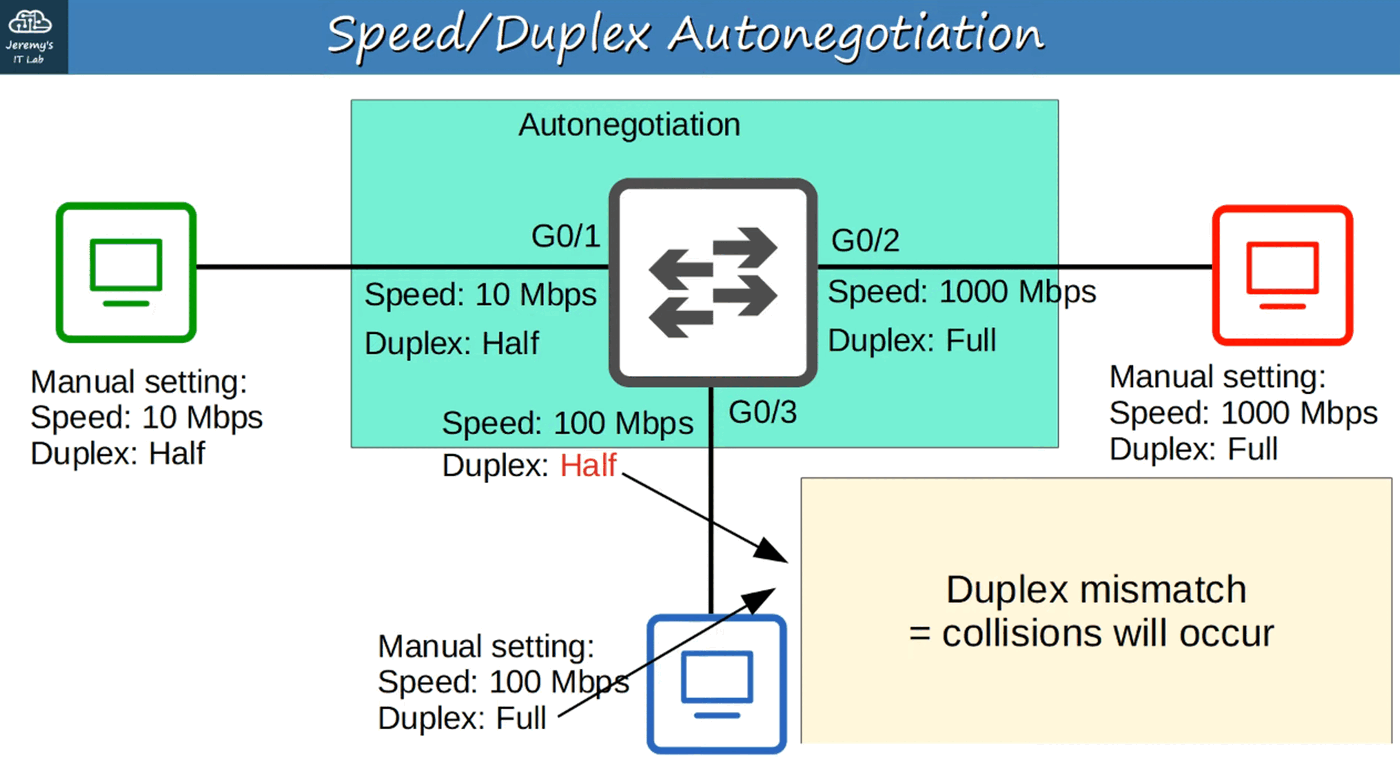
\includegraphics[keepaspectratio,alt={image}]{images/09-switch-interfaces/img-009.png}}
\end{figure}

\begin{itemize}
\tightlist
\item
  SPEED: The SWITCH will try to send at the speed that the other device
  is operating at. If it fails to send the speed, it will use the
  slowest supported speed (ie: 10 Mbps on a 10/100/1000 interface).
\item
  DUPLEX: If the speed is 10 or 100 Mbps the SWITCH will use HALF
  DUPLEX. If the speed is 1000 Mbps or great, it will use FULL DUPLEX.
\end{itemize}

\section{Interface Counters and
Errors}\label{interface-counters-and-errors}

Show using the:

// Privileged EXEC mode

SW1\#show interfaces \textless interface name\textgreater{}

Error stats will be at the bottom.

\begin{figure}
\centering
\pandocbounded{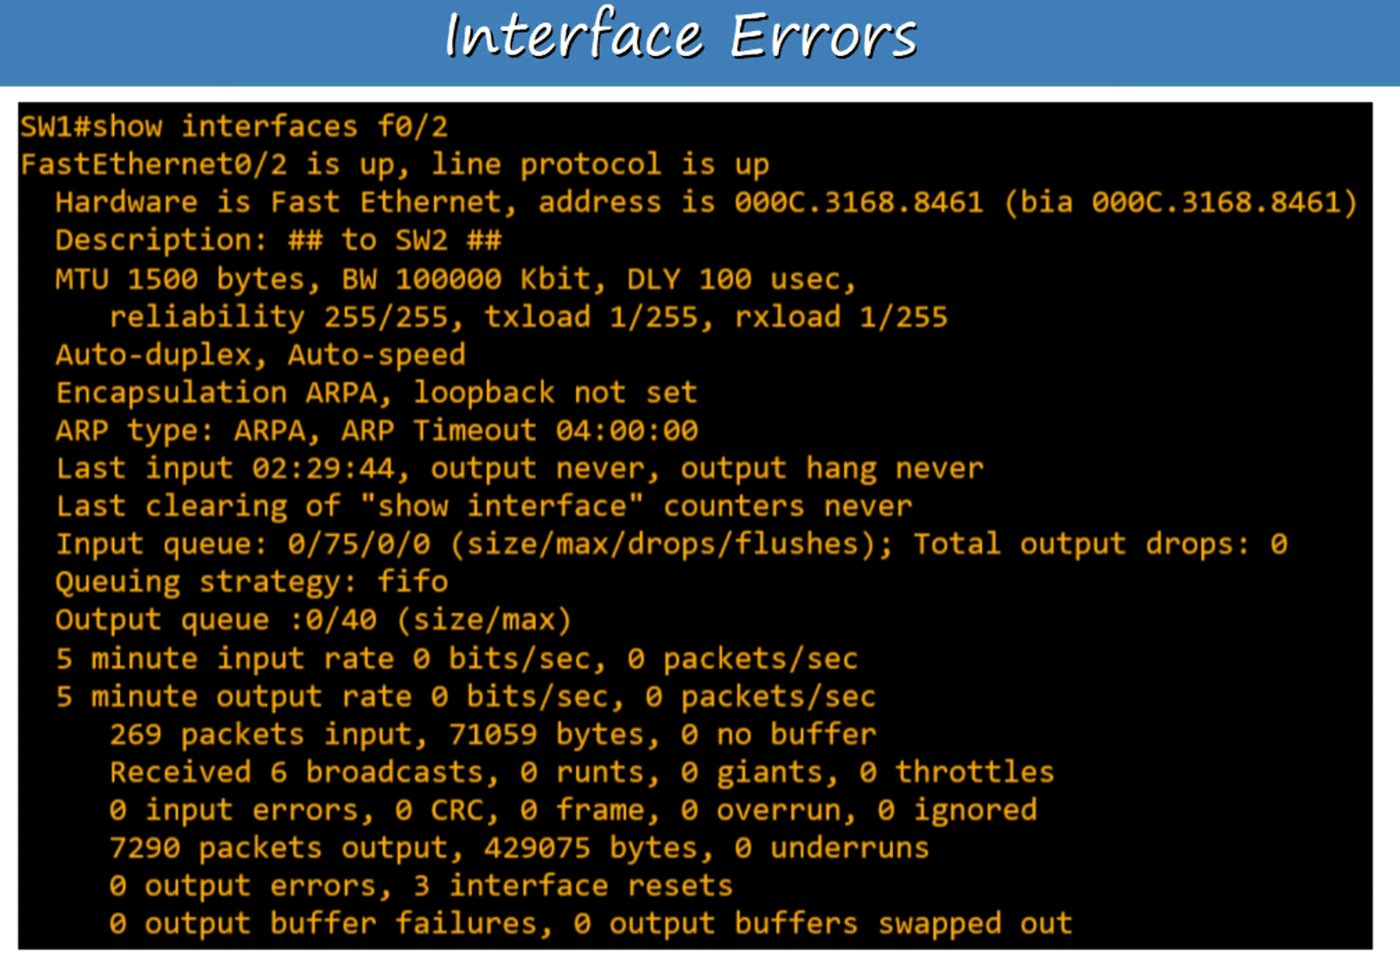
\includegraphics[keepaspectratio,alt={image}]{images/09-switch-interfaces/img-010.png}}
\end{figure}

\textbf{Packets Received / Total bytes received.}

\textbf{Runts}: Frames that are smaller than the minimum frame size (64
bytes)

\textbf{Giants}: Frames that are larger than the maximum frame size
(1518 bytes)

\textbf{CRC}: Frames that failed the CRC check (in the Ethernet FCS
trailer)

\textbf{Frame}: Frames that have an incorrect format (due to an error)

\textbf{Input errors}: Total of various counters, such as the above four

\textbf{Output errors}: Frames the SWITCH tried to send, but failed due
to an error
